\chapter{Parallelisierung}
\label{chp:para}

\section{Topologie}
\label{sec:topo}

Wir hatten anfangs beschlossen, dass mehrere Subpopulationen erzeugt
werden, die sich dann untereinander austauschen, wie in
Abbildung~\ref{fig:mult-subpop} beschrieben.

\begin{SCfigure}
  \centering
  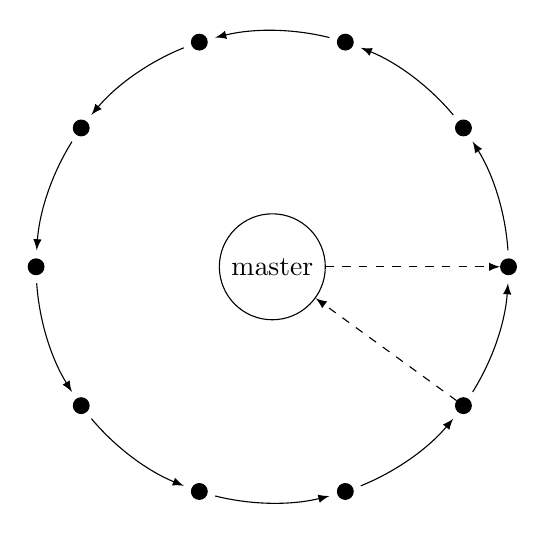
\begin{tikzpicture}
    [place/.style={circle,
      inner sep=0pt,minimum size=2mm}]
    %% from http://www.texample.net/tikz/examples/cycle/
    % Author : Jerome Tremblay
    \def \n {10}
    \def \radius {3cm}
    \def \margin {4} % margin in angles, depends on the radius

    \foreach \s in {1,...,\n}
    {
      \node[draw, circle, fill=black, place] (\s) at ({360/\n * (\s - 1)}:\radius) {};
      \draw[->, >=latex] ({360/\n * (\s - 1)+\margin}:\radius)
      arc ({360/\n * (\s - 1)+\margin}:{360/\n * (\s)-\margin}:\radius);
    }

    \node[draw, circle] (master) at (0:0) {master};
    \draw[->, >=latex, dashed] (master) -- (1);
    \draw[->, >=latex, dashed] (\n) -- (master);
  \end{tikzpicture}
  \caption[Mehrere Subpopulationen]{\label{fig:mult-subpop}Es werden mehrere Subpopulationen
    erzeugt, die dem jeweils nächsten Prozess dann Teile aus der
    eigenen Population zusenden.}
\end{SCfigure}

Dabei stießen wir aber auf mehrere Probleme.  Zum einen mussten wir
selber einen kleinen „garbage collector“ implementieren, der sich um
das Löschen von Graphen kümmern sollte.  Da dies aber asynchron
verlief, konnte es zu „race conditions,“ bei denen ein Graph gelöscht
wurde und danach ein Prozess diesen in die eigene Population aufnehmen
wollte, kommen.

Deshalb hatten wurde der Aufbau so verändert, dass der Hauptprozess
alle Kindprozesse instruiert jeweils einen „Offspring“ zu erzeugen und
diesen wieder zurückzuschicken
(vgl. Abbildung~\ref{fig:topology-central}).  Da in diesem Fall aber
die Population nur zentral verwaltet wurde, musste die Einsortierung
in die neue Population serialisiert %% this word does not really fit
geschehen, was der Nebenläufigkeit schadet.  Darüber hinaus konnte
während dieses Zeitraums der Status des Algorithmus nicht abgefragt
werden.

\begin{SCfigure}
  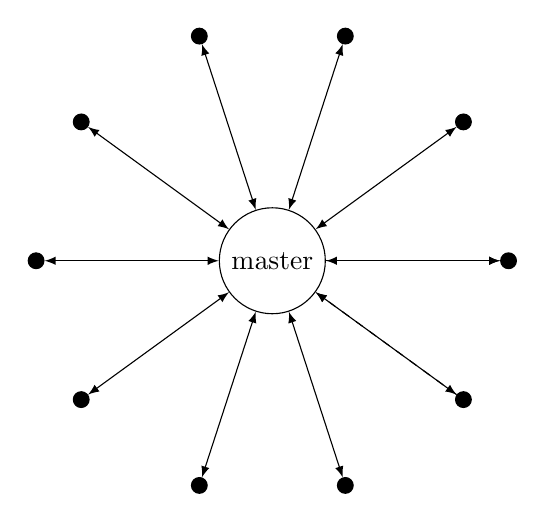
\begin{tikzpicture}
    [place/.style={circle,
      inner sep=0pt,minimum size=2mm}]
    \def \n {10}
    \def \radius {3cm}
    \def \margin {4} % margin in angles, depends on the radius

    \node[draw, circle] (master) at (0:0) {master};

    \foreach \s in {1,...,\n}
    {
      \node[draw, circle, fill=black, place] (\s) at ({360/\n * (\s - 1)}:\radius) {};
      \draw[<->, >=latex] (master) -- (\s);
    }

    \draw[->, >=latex, dashed] (master) -- (1);
    \draw[->, >=latex, dashed] (\n) -- (master);
  \end{tikzpicture}
  \caption[Verteilte Erzeugung von Offsprings]
  {\label{fig:topology-central} Die Kindprozesse erzeugen einzelne
    Rundreisen und schicken diese an den „master“ zurück.  Dieser muss
    die Rundreisen dann in die eigene Population einsortieren.}
\end{SCfigure}

\section{ets tables}
\label{sec:ets}

%% ets tables
Wir haben außderdem die Sprache zum Teil zweckentfremdet.  Das normale
Limit von Datenbanktabellen liegt bei 1400.  Da unsere Graphen aber
jeweils drei Stück besitzen, können wir unser Programm nicht beliebig
parallelisieren, da sonst das Limit auf einer Node erreicht wird.
Darüber hinaus werden diese nicht von der „garbage collection”
gelöscht sondern müssen manuell freigegeben werden.  Die Tabellen
haben allerdings immer einen Besitzer und nur dieser hat das Recht den
Speicher einer Tabelle aufzulösen.  Benutzen nun also mehrere Prozesse
die selben Tabellen, muss der Besitzer immer geändert werden.

% Das wird im Detail in Kapitel~\ref{chp:para} behandelt.
